% siminos/spatiotemp/chapter/QFTlatt.tex
% $Author: predrag $ $Date: 2021-12-24 01:25:20 -0500 (Fri, 24 Dec 2021) $

% input by catMapLatt.tex

% \renewcommand{\ssp}{\ensuremath{\phi}}             % lattice site field
\renewcommand{\shift}{\ensuremath{r}}
\renewcommand{\Xx}{\ensuremath{\mathsf{\Phi}}}      % kittens lattice field
\renewcommand{\Laplacian}{\square}
\renewcommand\speriod[1]{{\ensuremath{L_{#1}}}}  %continuous spatial period
\renewcommand\period[1]{{\ensuremath{T_{#1}}}}  %continuous time period
\renewcommand{\Tr}{\mbox{\rm Tr}\,}

\section{Lattice discretization of a field theory}
\label{sect:lattDisc}

% \newcommand{\field}{{\phi}}     % used in lattFT.tex

%%%%%%%%%%%%%%%%%%%%%%%%%%%%%%%%%%%%%%%%%%%%%%%%%%%%%%%%%%%%%%%%%%%%%%%%
% https://arxiv.org/abs/hep-lat/0012005
% Lattice Gauge Theory - A Short Primer
% G.~M\"unster and M.~Walzl\rf{MunWal00}
%%%%%%%%%%%%%%%%%%%%%%%%%%%%%%%%%%%%%%%%%%%%%%%%%%%%%%%%%%%%%%%%%%%%%%%%
    \PC{2020-03-15}{
Some of the formulas initially extracted from  G.~M\"unster and M.~Walzl\rf{MunWal00}
\emph{Lattice Gauge Theory - A Short Primer},
\arXiv{hep-lat/0012005}, to use in CL18\rf{CL18}

Maybe already used:
\bigskip

for CL18\rf{CL18}:

$\ssp_\ell = \ssp(a\ell)$, where
$\ssp(a\ell)$ is defined by the value of the continuum
field $ \ssp(\ssp)$ at the lattice point $\ssp_\ell=a\ell$

(Here we work in Euclidean space.)
    }

%%%%%%%%%%%%%%%%%%%%%%%%%%%%%%%%%%%%%%%%%%%%%%%%%
\begin{figure}
  \centering
  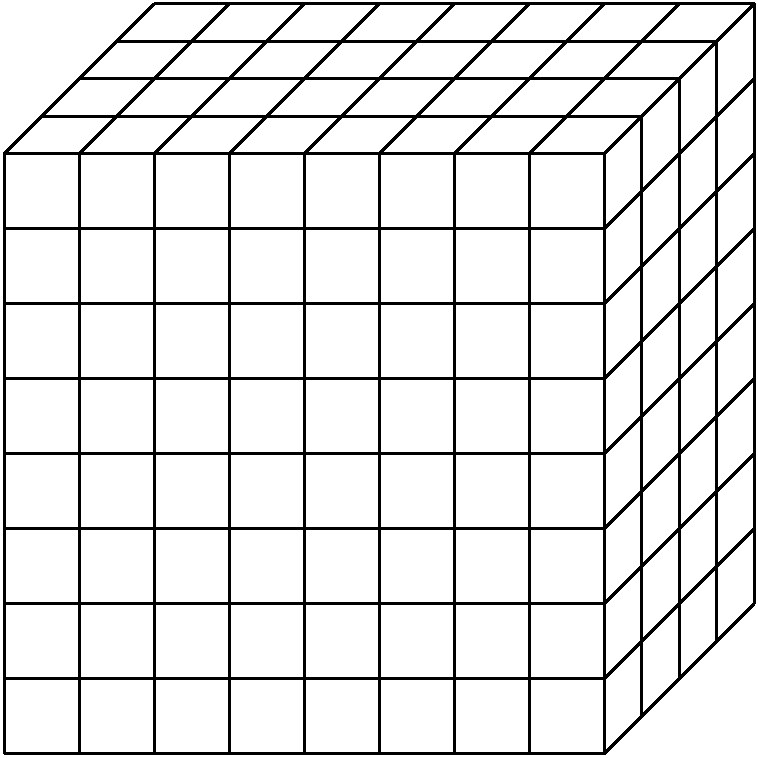
\includegraphics[width=0.5\textwidth]{MunWal00lattice}
  \caption{
3\dmn\ lattice. From \refref{MunWal00}.
  }\label{fig:MunWal00lattice}
\end{figure}
%%%%%%%%%%%%%%%%%%%%%%%%%%%%%%%%%%%%%%%%%%%%%%%%%

In Euclidean field theory the fields $\field(x)$ depend on the $d$ Euclidean
coordinates, so introduce a discretized spacetime in form of a
$d$-periodic hypercubic \emph{integer lattice} $\integers^d/\speriod{}^d$
(see \reffig{fig:MunWal00lattice}), with lattice spacing $a_{i}=\Delta
x_{i}$ and lattice period $\speriod{i}=1/\Delta x_{i}$ along the unit
vector
\[
\hat{n}_{i}
    \in
\left\{\hat{n}_1, \hat{n}_2, \cdots , \hat{n}_d\right\}
\]
pointing in the $i$th positive direction. The (scalar) \emph{field}
$\field(x)$ is evaluated only on the lattice points
\beq
\field_z
=
\field(x)
    \,,\qquad \qquad x = az= \mbox{lattice point}
    \,,\quad z \in \integers^d/\speriod{}^d
\,.
\ee{LattField}
It is periodic
\[
\field_z = \field_{z+\speriod{i}\hat{n}_{i}}.
\]
in all directions.
We refer to the set of values of $\Xx=\{\field_z\}$ as a {\em {\lattstate}}.
    \index{lattice!state}\index{lattice!configuration}

In order to discretize field-theoretic partial differential equations, we
need to {lattice derivatives}.
The  {\em forward partial lattice derivative}
    \index{lattice!derivative}\index{derivative, lattice}
    \index{lattice!derivative, forward}
\beq
(\partial_{i} \field)_z
        =
    \frac{\field(x+\Delta x_{i}{\hat{n}_{i}}) - \field(x)}{\Delta x_{i}}
        =
    \frac{\field_{z+{\hat{n}_{i}}} - \field_z}{\Delta x_{i}}
%\,.
\ee{latticePartDer}
depends explicitly on the lattice spacing. For our purposes it is
convenient to reformulate the problem as a discretization on
an integer lattice.
This is attained by converting all continuum partial \emph{derivatives}
into discrete partial \emph{differences} by
\(
\partial_{i} \to \speriod{i}\partial_{i}
\)
rescaling of the partial derivatives. After this rescaling $\partial_{i}$
is an integer lattice forward partial {\em difference operator}
\beq
\partial_{i} = \shift_{i}  - \unit
\,.
\ee{forwDer}
Higher lattice partial difference operators can be defined as\rf{Elaydi05}
\beq
\pde_{i}^k = \sum_{j=0}^k(-1)^j\,\combinatorial{k}{j}\,\shift_{i}^{k-j}
\,,
\label{Elaydi05(2.1.1)}
\eeq
with support on $k+1$ forward points. For example
\bea
\partial_{i}^2 &=& \shift_{i}^2  - 2\shift_{i} + \unit
            \continue
\partial_{i}^3 &=& \shift_{i}^3  - 3\shift_{i}^2  + 3\shift_{i} - \unit
\,.
\label{Elaydi05(2.1.1a)}
\eea
The even ones can be centered to be
reflection symmetric (symmetric under transposition) by translation by
$k$ sites,
\bea
\Laplacian_{i} &=&  - \transp{\partial}_{i}\partial_{i}
        \,=\, \shift_{i}  - 2\unit + \shift_{i}^{-1}
            \continue
\Laplacian_{i}^2 &=& \shift_{i}^2 - 4\shift_{i} + 6\unit  - 4\shift_{i}^{-1} + 6\shift_{i}^{-2}
\,,
\label{Box(2.1.1)}
\eea
where $\Laplacian=\sum\Laplacian_{i}$ stands for the lattice Laplacian
(or d'Alambertian).

Spacetime integrals are now replaced by sums,
\[
\int\!d^dx \quad \longrightarrow  \sum_x a^d
\,,
\]
    \PC{2020-03-15}{
\[
\partial_{\mu}\ssp(x) =
\frac{1}{a} (\ssp(x+a{\hat{\mu}})-\ssp(x)),
\]
and spacetime integrals by sums:
\[
\int\!d^4x \quad \longrightarrow  \sum_x a^4 \ .
\]
    }
and the lattice free field action is
\bea
S &=&
\sum_x a^d \left\{ \frac{1}{2} \sum_{i =1}^d
(\partial_{\mu}\field(x))^2 + \frac{\mu^2}{2}\field(x)^2
% + \frac{g_0}{4!}\field(x)^4
\right\}
\continue
 &=&
\sum_z a^d \left\{\frac{1}{2}\sum_{i =1}^d
\field_z\left(-\Laplacian_{i} + \mu^2\right)_{zz'}\field_{z'}
\right\}
\,.
\label{MunWal00freeAct}
\eea
In the functional integrals the measure
\[
{\cal D}\field  =  \prod_x d\field(x)
\]
involves the lattice points $x$ only, so for a finite lattice this is a
finite dimensional integral.

involves the lattice points $x$ only, so we have a discrete set
of variables to integrate. If the lattice is taken to be finite, we just
have finite dimensional integrals.

    \PC{2020-03-15}{
Let us assume a hypercubic lattice with length $L_1=L_2=L_3=L$ in
every spatial direction and length $L_4=T$ in Euclidean time,
\[
x_{\mu} = an_{\mu},\qquad n_{\mu} = 0,1,2,\dots,L_{\mu}-1,
\]
with finite volume $V = L^3T$, and periodic boundary conditions
\[
\ssp(x) = \ssp(x+aL_{\mu}\,\hat{\mu}),
\]
where $\hat{\mu}$ is the unit vector in the $\mu$-direction.
    }

The momenta are also discretized,
\[
p_{\mu} = \frac{2\pi}{a}\,\frac{l_{\mu}}{\speriod{\mu}}\qquad \mbox{with}\
l_{\mu} = 0,1,2,\dots,\speriod{\mu}-1,
\]
and the momentum-space integration is replaced by finite sums
\[
\int\!\frac{d^4p}{(2\pi)^4}\ \longrightarrow \
\frac{1}{a^4 \speriod{}^3 T}\sum_{l_{\mu}}
\,.
\]
All ``functional integrals'' are now regularized, finite
expressions.

To recover physics in a continuous and infinite spacetime, one needs to
take the infinite volume limit,
\[
\speriod{},T \longrightarrow \infty
\,,
\]
and the continuum limit,
\[
a \longrightarrow  0.
\]
We shall not discuss the continuum limit of a lattice field theory here.

\subsection{Transfer matrix}
\label{sect:transfMat}

Picking out a `time direction' and evolving in time slices (what we call
Hamiltonian formulation) is here called `transfer matrix', presumably in
reference to the similar formulation for the Ising model.

Split the 4D hypecubic lattice $z=(z_1,z_2,z_3,z_4)$ into 3\dmn\
`spatial' directions $\textbf{z}=(z_1,z_2,z_3)$ and the `temporal'
direction $z_4=\zeit$.
Let
\beq
\Xx_\zeit = \{\field_z | z_4=\zeit\}
\ee{MonMun94:(1.184)}
be a  field configuration on a Euclidean time slice $z_4=\zeit$.
Decompose the lattice action as
\beq
S[\field] = \sum_\zeit L[\Xx_{\zeit+1},\Xx_\zeit]
\ee{MonMun94:(1.185)}
This sum looks like the usual 1D temporal lattice action \refeq{MacMei83-4}.
Here
\beq
L[\Xx_{\zeit+1},\Xx_\zeit]=
          \sum_{\textbf{z}}\frac{1}{2}(  \field_{\textbf{z},\zeit+1}
                                        -\field_{\textbf{z}\zeit}   )^2
        + \frac{1}{2}(L_1[\Xx_\zeit] + L_1[\Xx_{\zeit+1}])
\ee{MonMun94:(1.186)}
with (here I drop a non-harmonic potential terms)
\beq
L_1[\Xx_\zeit]=
          \sum_{\textbf{z}}\frac{1}{2}
           \left\{\sum_{k=1}^3(\field_{\textbf{z}+\hat{k},\zeit}
                               -\field_{\textbf{z}\zeit})^2
                                + \frac{m^2}{2}\field_{\textbf{z}\zeit}^2
           \right\}
\ee{MonMun94:(1.187)}
Eq.~\refeq{MonMun94:(1.186)} looks like a sensible generalization of the
temporal lattice generating function \refeq{MKMP84(3.6)}.

The transfer matrix is defined as
\beq
T[\Xx_{\zeit+1},\Xx_\zeit]=
        e^{-L[\Xx_{\zeit+1},\Xx_\zeit]}
\ee{MonMun94:(1.188)}
As the matrices are presumably not commuting,
it is not obvious to me that repeated application of the
transfer operator adds up to the lattice action $S[\field]$
\refeq{MonMun94:(1.185)} in the exponent.
Take a field $\Psi_\zeit$ defined on $\zeit$ time-slice. Then the
transfer operator evolves the initial time-slice by matrix multiplication,
\beq
T^\cl{}\Psi_\zeit=\Psi_{\zeit+\cl{}}
\ee{MonMun94:(1.189)}
As it stands, it is not obvious how this is supposed to work, but Montvay
and M{\"u}nster\rf{MonMun94} do give the standard differential
formulation, explain correlations, \etc, so it's probably OK. For a
time-periodic lattice of time period $\period{}$ they say that
\beq
Z= \Tr T^\cl{}
\ee{MonMun94:(1.196)}
is the \emph{partition function}.

\begin{description}
  \item[2020-07-04 Predrag]
Would be happier if \refeq{MonMun94:(1.196)} were a $\Det$,
\ie, if there were a
\(
T=1-zJ
\)
kind of expression. But ...
I do not see a quick way from here to the Hill's formula, so I abandon
this path for now.
\end{description}

\subsection{Classical {$\phi^3$} lattice field theory}
\label{sect:phi3latt}

\begin{description}
  \item[2021-12-23 Predrag]
All {$\phi^k$} lattice field theories fit under the ``generalized
\HenonMap'' umbrella, so {$\phi^3$}, {$\phi^k, k>4$} are covered in
\refsect{sect:HamHenonMap}~{\em {\Henlatt}; anti-integrable limit}

\end{description}

\subsection{Classical {$\phi^4$} lattice field theory}
\label{sect:phi4latt}

Field theorists do not like odd potentials, such as the {\henlatt}
\refeq{henlattBWcubic}, as they are not bounded from below.

We should be able to write \refeq{phi4actionSch} action
$S[\Xx]$ such that the derivative of the quartic term yields classical
{$\phi^4$} theory \refeq{KarZar12(69)} on $d$\dmn\ lattice
\beq
-\ssp_{\zeit+1} + \frac{g}{3!}\ssp_{\zeit}^3 - \ssp_{\zeit-1} = \Ssym{\zeit}
\,.
\label{phi4-1dLatt}
\eeq
To get some intuition, find the 3 steady states $\ssp_{\zeit}=\ssp$
by plotting
\beq
V'[\ssp] = 2\ssp  - \frac{g}{3!}\ssp^3 = 2\,\ssp(1 - \frac{g}{12}\ssp^2)
%\,,
\ee{phi4pot-1dLatt}
as a function of (sufficiently strong) stretching $g$, and then picking a
sensible constant source $\Ssym{\zeit}=\Ssym{}$ value
(or 3 values $\Ssym{\zeit}\in\{L,C,R\}$, see \refexam{exam:ReflectA}~{\em
A reflection--symmetric  $1d$ map.})
for which not only the 3 fixed points  are real, but all $3^\cl{}$
3-symbol bimodal map itineraries are realized.

Continued around \refeq{phi4antiInteg}.

\bigskip

The \HillDet\ $\|\jMorb[\Xx]\|$ is again of the same form
\refeq{jMorb1dField}, with the stretching factor at site $\zeit$
depending on the coupling constant ${g}$, the lattice site field for the
given \lattstate.

For example, the {\HillDet} of the $[4\times4]$ \jacobianOrb\ $\jMorb$ is
({\color{red}correct this!}):
\bea
\Det(\jMorb)
&=&
\left\|
\begin{array}{cccc}
 {s}_1 &-1 & 0 &-1  \\
-1 & {s}_2 &-1 & 0 \\
 0 &-1 & {s}_3 &-1 \\
-1 & 0 &-1 & {s}_4
\end{array}
\right\|
     \label{HillDet4x4}\\   % was {LC21:HLdetCycD8s1}
&=&
  {s}_1 {s}_2 {s}_3 {s}_4 +{s}_1 {s}_2 {s}_3
+ {s}_2 {s}_3 {s}_4
\ceq
 +{s}_1 {s}_2
 +{s}_2 {s}_3
 +{s}_1 {s}_4
 +{s}_3 {s}_4 +{s}_1 +{s}_2 +{s}_3 +{s}_4
   \,.
\nnu
\eea

\begin{description}


\PCpost{2016-08-20}{
Might be worth a look - several papers on coupled map lattices, see
also \refref{HooAok16} on order and chaos in a continuous time,
1\dmn\ latticel $\phi^4$
model - if you read that literature, please share what you have learned
by writing it up there.
    }

\item[2021-08-11 Predrag]

Karimipour and Zarei\rf{KarZar12}
{\em Completeness of classical {$\phi^4$} theory on two-dimensional lattices}
\arXiv{1201.4558}:

The 2\dmn\ $\phi^4$ Hamiltonian for all discrete scalar field theories on
a two dimensional square lattice with periodic boundary conditions
\beq
  H_c=
  \sum_{\langle r,s\rangle}K_{r,s}(\phi_r-\phi_s)^2
  +\sum_{r}h_r \phi_r +m_r \phi_r^2+ q_r \phi_r^4,
\ee{KarZar12(69)}
where $K_{r,s}\in \{i,-i\}, \ i=\sqrt{-1}$ and the real
parameters $h_r$, $m_r$ and $q_r$ denote respectively the
inhomogeneous external field, the quadratic (mass term) and
quartic coupling strengths. The linear terms $\{h_r\}$ are also
necessary for completeness.

From
\HREF{http://www.scholarpedia.org/article/Triviality_of_four_dimensional_phi\%5E4_theory_on_the_lattice}
{Scholarpedia}:
action
\beq
S = \sum_z \left[ \varphi_z^2 + \lambda \left( \varphi_z^2 - 1 \right)^2 \right]
    - 2 \kappa \sum_{\langle z z' \rangle} \varphi_z \varphi_{z'}
\,.
\ee{phi4actionSch}


\item[2021-12-05 Predrag]
$\phi^4$ theory also shows up in Br{\'e}zin \& Zinn-Justin
(see \refsect{sect:MFT-Ising}) {\em Mean field theory for the Ising model}.
Their formulation suggests that the partition function \refeq{partFunct} should be
written as \refeq{NKHM15cw} where $f[\Xx]$ is free energy (the
large-deviation potential)
\beq
Z[\source]	= e^{-{N_\lattice} f[\source]}
\,.
\ee{NKHM15ZJ}
and $N_\lattice$ is the number of lattice sites.

\item[2021-12-07 Predrag]

Vierhaus's masters thesis\rf{Vierhaus10} {\em Simulation of {$\phi^4$}
theory in the strong coupling expansion beyond the {Ising} Limit}
has a clear discussion of the
\HREF{https://edoc.hu-berlin.de/bitstream/handle/18452/14790/vierhaus.pdf?sequence=1&isAllowed=y\#section.2.3}
{Ising limit of {$\phi^4$}}.
Note the reformulation \refeq{phi4actionSch} of the action, his eq.~(2.15).

\item[2021-12-21 Predrag]
Hagiwara and Shudo\rf{HaShu04a}
{\em An algorithm to prune the area-preserving {H{\'e}non} map}
(2004)
describes Sterlings anti-integrable method.

Starting with the \henlatt\ second-order difference equation
\refeq{Hen-1dLattA}, changing
variables to $z = \epsilon x$, $\epsilon = a^{-1/2}$ gives
\beq
-\epsilon(z_{\zeit-1}+z_{\zeit+1}) + z_\zeit^2 - 1 = 0
\,.
\ee{HaShu04a(2)}
At the anti-integrable limit $\epsilon\to0$, the map
reduces to $z_\zeit^2 = 1$,
with every orbit an arbitrary sequence of $\pm1$.

\item[2021-12-22 Predrag] An unchecked reverse engineering guess:
Starting with the second-order difference equation for
$\phi^4$ theory:
\beq
-\epsilon(z_{\zeit-1}+z_{\zeit+1}) + z_\zeit(z_\zeit-1)(z_\zeit+1) = 0
\,.
\ee{phi4antiInteg}
At the anti-integrable limit $\epsilon\to0$, the map
reduces to $z_\zeit(z_\zeit-1)(z_\zeit+1)= 0$,
with every orbit an arbitrary sequence of $\{-1,0,1\}$.
Then go back to \refeq{phi4-1dLatt}, using
$\ssp= z/\epsilon$, $\epsilon = g^{-1/3}$.
\beq
- \ssp_{j-1} + g\,\ssp^3_j - \ssp_{j+1} =  g^{2/3}\ssp_j
\,.
\ee{PCphi4}
Probably not the right thing; note that
\refeq{Anastassiou21(6)} scales the linear term differently,
 by $\epsilon$.

\item[2021-12-22 Predrag]
Anastassiou, Bountis and B{\"a}cker\rf{AnBoBa17} {\em Homoclinic points of
{2D} and {4D} maps via the parametrization method} (2017):

the dynamics of discrete breather solutions on
1--dimensional
lattices (or chains) of nonlinearly interacting particles

The discrete nonlinear Klein-Gordon
system of ordinary differential equations
\beq
\ddot u_n=-V^\prime\left(u_n\right)+\alpha\left(u_{n+1}-2u_n+u_{n-1}\right)
\,, \quad
V(x)=\frac{1}{2}Kx^2+\frac{1}{4}x^4
\,,
\ee{AnBoBa17eq4}
where $u_n$ for $-\infty<n<\infty$ is the amplitude of the $n$-th
particle, $\alpha>0$ is a parameter indicating the strength of coupling
between nearest neighbors, and $V(x)$ is the on-site potential with
primes denoting differentiation with respect to the argument of $V(x)$.

Discrete nonlinear Schr{\"o}dinger equation is similar.


\item[2021-12-22 Predrag]
Must study Anastassiou\rf{Anastassiou21}
{\em Complicated behavior in cubic {H{\'{e}}non} maps},
(2021).
He defines the generalized \HenonMap\ of the plane onto itself as
\beq
H\colon \mathbb{R} ^2\to \mathbb{R} ^2,\qquad H(x,y)=(y, b\,x+p(y)),
\ee{Anastassiou21(3)}
The determinant of the Jacobian matrix connected to the dissipation of
the system is equal to $-b$. If the polynomial p(y) is odd, then the
map $H(x,y)$ is symmetric under the transformation
\beq
\sigma(x,y)=(-x,-y)
\,.
\ee{Anastassiou21(3a)}
For $-b=1$, the map is a symplectomorphism (or symplectic map)
because it preserves the natural symplectic form of the plane,
$dx\wedge{dy}$.

The dynamics of $H(x,y)$, where p(y) is a third-degree polynomial, was
studied in \refref{DulMei00}, sufficient conditions for hyperbolicity in
generalized {\HenonMap}s for arbitrary polynomials p(y) were given in
\refref{Zhang10}. Anastassiou studies cubic polynomial $p(y)$
{\HenonMap}s,
\beq
H\colon \mathbb{R} ^2\to \mathbb{R} ^2,\qquad H(x,y)
=\bigl(y,-b\,x+ g(y^3-y)\bigr),
\ee{Anastassiou21(4)}
studied from a different perspective in his earlier
articles\rf{AnBoBa17,AnBoBa18}. He locates the region of the \statesp\
\beq
\mathcal{A} =
\biggl\{(x,y)\in \mathbb{R} ^2\colon\,
 |x|,|y|\le \sqrt{1+\frac{2}{g}}\,\biggr\}
\,,
\ee{Anastassiou21(4a)}
where the bounded  nonwandering invariant set exists, and finds parameter
values \(g>4\) for which this nonwandering set is hyperbolic. Read his
proof - it is instructive.
% For this, he uses a classical result of Afraimovich et al.[13].
Remember that these are just very crude bounds - the stable/unstable
manifolds will give tight bounds.
He shows that his map is conjugate to the Bernoulli three-shift, using
the anti-integrability technique\rf{aub95ant,Chen04,BolMac97,BaChMa13}.
\[
-\ssp_{n+1} + g\,\ssp_{n}^3  -g\,\ssp_{n} - \ssp_{n-1}=0
\,,
\]
Define $\epsilon =1/g$
\beq
- \epsilon(\ssp_{n+2} + \ssp_{n+1}) + \ssp_{n+1}^3=\epsilon \,\ssp_n
\,,
\ee{Anastassiou21(6)}

It is customary to say that such a complex behavior is `chaotic' because
of Devaney's definition\rf{BBCDS92}.

\item[2021-06-04 Predrag]
Friedland and Milnor\rf{FriMil89}
{\em Dynamical properties of plane polynomial automorphisms} (1989)
introduced the generalized \HenonMap. Their theorem 2.6 on the normal
form of such maps is nice. In their fig.~2 they do the 0th order version
of the plot I hope Harrison and Ibrahim will plot: the three-fold
horseshoe associated with a real cubic polynomial.
Dullin and Meiss\rf{DulMei00} do that, their fig.~13\,(right).

\item[2021-06-04 Predrag]
See also Anastassiou, Bountis and B{\"a}cker\rf{AnBoBa18} (2018)
{\em {Recent results on the dynamics of higher-dimensional {H{\'{e}}non} maps}},
their fig.~1. They take
\beq
p(y) = cy + 3y^3
\ee{AnBoBa17}
They chose $c=-\frac{5}{2}$ throughout their publication (we should too,
to compare results).
``This choice is pictorially convenient, since $c$ values in that range
produce large scale manifolds that are clearly visible in the figures.''

The cubic mapping possesses three fixed points: saddle point at the
origin, for all parameter values, a symmetric pair at
\[
\left(\pm\sqrt{(2-c)/3},\pm\sqrt{(2-c)/3}\right)
\,.
\]
The $(0,0)$ fixed point Floquet multipliers are
\begin{equation}
   \frac{1}{2}\left(c-\sqrt{c^2-4}\right),
   \frac{1}{2}\left(c+\sqrt{c^2-4}\right)
   \,.
\end{equation}
Since $c=-5/2$ and $\delta=1$, the Floquet multipliers of the origin are
$\ExpaEig_u = -2$ and $\ExpaEig_s = -1/2$
with normalized eigenvectors
$(-1/\sqrt{5}, 2/\sqrt{5})$ and $(-2/\sqrt{5}, 1/\sqrt{5})$.
The origin is thus a saddle, with a 1--dimensional stable and a 1--dimensional
unstable manifold, whose parametric computation they explain.

\item[2021-06-04 Predrag]
Dullin and Meiss\rf{DulMei00}
{\em Generalized {H{\'{e}}non} maps: the cubic diffeomorphisms of the plane}
(2000):

 The Euler–Lagrange equation associated with this action is
\beq
 m(\ssp_{\zeit-1}+ \ssp_{\zeit+1}) =U'(\ssp_{\zeit})
\ee{DulMei00(20)}
which is the Lagrangian form of the \HenonMap.
They concentrate on the area-preserving cubic maps. [...]
These are reversible and have an additional symmetry on a codimension-one
line in parameter space (Predrag currently calls that `dynamical symmetry').

\item[2021-06-04 Predrag]
The Arneodo–Coullet–Tresser maps (referred to in \rf{LiMal04}) are
5-term recurrence equations with $\ssp_\zeit^k$ nonlinear term, ignore for now.

Li and Malkin\rf{LiMal04}
   {\em Bounded nonwandering sets for polynomial mappings} (2004)


\end{description}


%\newpage
\section{Normalizing flows}
\label{sect:discFTblog}

\textbf{Predrag}: What is here called

   `normalizing flow' \(f: \mathcal{X} \rightarrow \mathcal{X}\),
  invertible and differentiable

  Jacobian factor \(J(z) = |\det \partial f_i(z) / \partial z_j|\)

\noindent
is the main
idea of our \refrefs{conjug_Fred,CFTsketch}); what they call their
`latent' space probability distribution being set to Gaussian is what we
call `free field theory'. One pays a determinant of the Jacobian matrix
of that field transformation, the same as for us. But Miranda Cheng says
that this determinant ``can be easily computed/approximated" which is
news to me.

\begin{description}


\item[2021-11-01 Predrag]
 Miranda Cheng \\
\videoLink{YouTube.com/embed/%
Ff_jllXzMfk}
{\em Machine learning and theoretical physics: some applications}.

Lattice field theory is the main tool for doing nonpertubative
calculations in field theory.
The idea of ML techniques, such as Normalizing Flows, is that if we can
learn an invertible map that trivializes an interacting model to a free
theory, we can easily sample the latter and push back the samples through
the inverse map to obtain (proposed) samples from the original
non-trivial distribution.

\textbf{Predrag}: this is the main idea of our \refref{conjug_Fred,CFTsketch});
what they call their `latent' space probability distribution being set to
Gaussian is what we call `free field theory'. One pays a determinant of the
Jacobian matrix of that field transformation, the same as for us. But she says
that this determinant ``can be easily computed/approximated" which is news to me.

In the talk she defines the ``observable'' the way we would; I have not
seen the definition yet in their papers.

The first part is based on

Pim de Haan, Corrado Rainone, Miranda Cheng and  Roberto Bondesan%\rf{dRCB21}
{\em Scaling Up Machine Learning For Quantum Field Theory with
Equivariant Continuous Flows}, \arXiv{2110.02673}.
Cheng has typos in her presentation (probability density
$"+"\Det|J|$ rather than $\times$).

the contributions of their paper:
\vspace{-7pt}
\begin{itemize}
    \item They extend %\cite{pmlr-v119-kohler20a}
    and develop continuous normalizing flows for lattice field theories
    that are fully equivariant under lattice symmetries as well as the
    internal $\phi \mapsto -\phi$ symmetry of the $\phi^4$ model.
    \item They train our model for the $\phi^4$ theory and and for the
    $32\times 32$ lattice we improve the effective sample size from 1\%
    to 66\% w.r.t.~a real NVP baseline of similar size.
    % 5(Fig.~\ref{fig:results}).
    \item They study equivariance violations of real NVP models and
    contrast it with the exact equivariance of our flows.
\end{itemize}


If the vector field $g$ is equivariant, the resulting distribution on
$\phi$ is invariant. They show how to construct a $g$ equivariant to the
square lattice symmetries.

\paragraph{The $\phi^4$ theory}
possesses non-trivial symmetry properties and a phase
transition. In the case of $\phi^4$ theory in two dimensions, the {\em
field configuration} is a real function on

the vertex set $V_L$ of the square lattice

with periodic boundaries and size $L\times L$: $\phi: V_L \to
{\mathbb R}$.
The $\phi^4$ theory is described by a probability density
\beq
p(\phi) = \exp(-S(\phi))/Z
\,,
\ee{dRCB21probField}
with action
\beq
S(\phi) = \sum_{x,y\in V_L}\phi(x) \Delta_{x,y} \phi(y) + \sum_{x\in V_L}m^2\phi(x)^2 + \mathit{\lambda}\phi(x)^4
\label{dRCB21eq:S}
\eeq
Here $\Delta$ is Laplacian matrix of the square lattice $({\mathbb
Z}/L{\mathbb Z})^{\times 2}$, $m$ and $\lambda$ are numerical parameters.
In the case of this and other non-trivial field theoretical densities,
%direct sampling is impossible due to the statistical correlation between
%degrees of freedom spatially separated up to the \emph{correlation
%length} of the theory, a fundamental quantity denoted as $\xi$;
$Z$ is the normalisation factor that is not known analytically for $\lambda\neq 0$.

  Probability densities over those \statesp\ manifolds:

  \begin{itemize}
  \item
    Prior density \(r(z)\)
  \item
    Model density \(q(x)\)
  \item
    Target density \(p(x)\)
  \end{itemize}




Note that, besides the space-time symmetries of the periodic lattice,
the theory possesses a

discrete global symmetry $\phi \mapsto -\phi$.

We
shall choose the couplings in such a way that only one minimum of the
action, invariant under this symmetry, exists. See
[??] %\cite{hackett2021flowbased}
for relevant work in the case of a symmetry-broken case.

(Was commented out:)
We will work in the ``unbroken" phase with $m^2>0$,
%\MC{actually, $m^2$ is negative as we report in the table},
where the minimum of the action is
invariant under the global symmetry.
See \arXiv{2107.00734} for relevant work in the broken phase.

The periodic lattice $V_L$ has spatial symmetry group $G=C_L^2 \rtimes
D_4$, the semi-direct product of two cyclic groups $C_L$ of translations
and dihedral group $D_4$ of right angle rotations and mirrors.
To ensure spatial equivariance of the vector field model, we should have
that

$\forall g \in G, x,y,a, f, W_{g(x)g(y)af}=W_{xyaf}$.

Using the translation subgroup, we can map any point $x$ to a fixed point
$x_0$. This allows us to write $W_{xyaf}=W_{x_0t_x(y)af}$, $t_x(y) = y -
x + x_0$.

(Predrag - they seem to be defining the point group here:)\\
Then let $H\simeq D_4$ be the subgroup of $G$ such that $g(x_0)=x_0$ for
all $g\in G$, and denote the orbit of $y$ under $H$ by $[y]=\{y' \mid
\exists g \in H, g(y)=y'\}$.

For each such orbit $[y]$ and dimension $a$
and $f$, a free parameter $W_{[y]af}$ exists, so that the other
parameters are generated by $W_{xyaf}=W_{[t_x(y)]af}$.


(Was commented out; Predrag - they ignore symmetric lattice states here:)\\
As most orbits are of size 8, the number of free parameters per $a$ and
$f$ is approximately $L^2/8$.

The orbits of $D_4$, leaving point $(0, 0)$ invariant, for $L=16$ are
shown in Fig.~4. %\ref{fig:orbits} in the Appendix
For each color in that figure, for each
dimensions $a$ and $f$, we have a free parameter.\\
(Predrag - that figure says the 1/8th fundamental domain tiles
the square lattice, and ignores the symmetry boundaries. The ``free parameter''
is just the values of the field in the fundamental domain.)


\item[2021-12-05 Predrag]
These papers seem to be more informative:

Rezende and Mohamed  (2015) ``normalizing flows''
\arXiv{1505.05770}
\\
cites   Jordan,  Ghahramani,  Jaakkola  and Saul\rf{JGJS99}
{\em An introduction to variational methods for graphical models} (1999)

Del Debbio, Rossney and Wilson {\em Efficient Modelling of Trivializing
Maps for Lattice $\phi^4$ Theory Using Normalizing Flows: A First Look at
Scalability} \arXiv{2105.12481}

\item[2021-12-05 Predrag]
%@misc{albergo2021introduction,
Albergo, Boyda, Hackett, Kanwar, Cranmer, Racanière,
Jimenez Rezende and Shanahan, %\rf{ABHKCRJS21}
{\em Introduction to Normalizing Flows for Lattice Field Theory}
(2021),
\arXiv{2101.08176}:

      This notebook tutorial demonstrates a method for sampling Boltzmann
      distributions of lattice field theories using a class of machine
      learning models known as normalizing flows. The ideas and
      approaches proposed in

\arXiv{1904.12072}

\arXiv{2002.02428}

\arXiv{2003.06413}

      are reviewed and a concrete implementation of the
      framework is presented. We apply this framework to a lattice scalar
      field theory and to U(1) gauge theory, explicitly encoding gauge
      symmetries in the flow-based approach to the latter.

%@article{PhysRevLett.125.121601,
%  title = {Equivariant Flow-Based Sampling for Lattice Gauge Theory},
%  author = {Kanwar, Gurtej and Albergo, Michael S. and Boyda, Denis and Cranmer, Kyle and Hackett, Daniel C. and Racani\`ere, S\'ebastien and Rezende, Danilo Jimenez and Shanahan, Phiala E.},
%  journal = {Phys. Rev. Lett.},
%  volume = {125},
%  pages = {121601},
%  year = {2020},
%  doi = {10.1103/PhysRevLett.125.121601},
%}

The Box-Muller transform is an example of a `normalizing' transformation:
to produce Gaussian random variables, draw two variables \(U_1\) and
\(U_2\) from \(\text{unif}(0,1)\), then change variables to
\beq
    (Z_1,Z_2) = (r\,\cos(2\pi U_2),\,r\,\sin(2\pi U_2))
\,,\qquad r= \sqrt{-2 \ln{U_1}}
\,.
\ee{ABHKCRJS21(1)}
The resulting variables \(Z_1, Z_2\) are then distributed according to
an uncorrelated, unit-variance Gaussian distribution; $U_1$ controls the
radius, and $U_2$ the angle of a $2d$ Gaussian.
\\
{\bf Predrag}: {\color{red}
This might relate Bernoulli and \templatt\ to Gaussian field theories
(see \refsect{sect:GaussianModel}), \ie, this maps fields in $[0,1)$
to fields in $\reals$.
                }

The density associated with output samples is computed
by the \emph{change-of-variables formula} relating the \emph{prior
density} \(\rho(U_1, U_2) = 1\) to the \emph{output density}
% \(q(Z_1, Z_2)\):
\beq
\begin{split}
    q(Z_1, Z_2) &= \rho(U_1, U_2) \left|
    \det\frac{\partial Z_k(U_1, U_2)}{\partial U_l} \right|^{-1} \\
    &= 1 \times \left| \det \left( \begin{matrix}
        \frac{-1}{U_1 r} \cos(2\pi U_2) &
        - 2\pi r \sin(2\pi U_2) \\
        \frac{-1}{U_1 r} \sin(2\pi U_2) &
        2\pi r \cos(2\pi U_2)
        \end{matrix} \right) \right|^{-1} \\
    &= \left| \frac{2 \pi}{U_1} \right|^{-1}.
\end{split}
\ee{ABHKCRJS21(2)}
\(J(U_1,U_2)\equiv\det({\partial Z}/{\partial U})\)
is the determinant of the Jacobian
of the coordinates transformation \((U_1,U_2)\to(Z_1,Z_2)\). The Jacobian
factor is a change in volume element, therefore the change-of-variables
formula must contain the inverse of this factor (spreading out volume
decreases density). As
\[U_1 = \exp(-(Z_1^2 + Z_2^2) / 2)\] and the initial density $\rho(U_1,U_2)$
over the unit square was uniform, the transformed density is
\beq
    q(Z_1, Z_2) = \frac{1}{2\pi} e^{-(Z_1^2 + Z_2^2)/2}
\,.
\ee{ABHKCRJS21(3)}
This example has no free parameters because no extra parameters were needed
to create a transform that exactly reproduced the desired target
distribution, independent, unit-variance Gaussian. In general, we may not
know a normalizing flow that exactly produces our desired distribution,
and so instead construct parametrized models that we can variationally
optimize to \emph{approximate} that target distribution, and because we
can compute the density these can be corrected to nevertheless guarantee
exactness.

In some cases, it is easy to compute the Jacobian factor even when the
whole Jacobian matrix is intractable; for example, only the diagonal
elements are needed if the Jacobian matrix is known to be triangular.

The hypercubic lattice discretization of the derivatives of the continuum
Euclidean action gives rise to a lattice Euclidean action,
\beq
\begin{split}
S^E_{\text{cont}}[\phi] &=
\int d^2\vec{x} ~ (\partial_\mu \phi(\vec{x}))^2 + m^2 \phi(\vec{x})^2
                  + \lambda \phi(\vec{x})^4
\\
\rightarrow
S(\phi) &= \sum_{\vec{n}} \phi(\vec{n})
    \left[ \sum_{\mu \in \{1,2\}}
      - \phi(\vec{n}+\hat{\mu}) + 2\phi(\vec{n})  - \phi(\vec{n}-\hat{\mu})
    \right]
    + m^2 \phi(\vec{n})^2 + \lambda \phi(\vec{n})^4
\end{split}
\ee{ABHKCRJS21(11)}
where now \(\phi(\vec{n})\) is only defined on the sites
of the \(L_x \times L_y\) lattice, \(\vec{n} = (n_x, n_y)\), with
integer \(n_x, n_y\).
% We have implicitly moved to ``lattice units'' where \(a=1\) such that
% \(L_x, L_y, V\) are integers and all quantities are unitless.
The discretized field \(\phi\) can be thought of
as an \((L_x \times L_y)\)-dimensional vector. We use periodic boundary
conditions in all directions, i.e.~\(\phi(L_x, y) \equiv \phi(0, y)\),
etc.

More details on \(\phi^4\) lattice scalar field theory can be found in
%\cite{vierhaus2010simulation}.
%
% 2010-07-27 Diplomarbeit
Vierhaus's masters thesis\rf{Vierhaus10} {\em Simulation of {$\phi^4$}
theory in the strong coupling expansion beyond the {Ising} Limit}.
%\HREF{https://doi.org/10.18452/14138} {DOI: 10.18452/14138}.

  The lattice action then defines a probability distribution over
configurations \(\phi\), \begin{equation}
p(\phi) = \frac{1}{Z} e^{-S(\phi)}, \quad
Z \equiv \int \prod_{\vec{n}} d\phi(\vec{n}) ~ e^{-S(\phi)},
\end{equation} where \(\prod_{\vec{n}}\) runs over all lattice sites
\(\vec{n}\). This is the distribution we are training the normalizing
flows to reproduce. While \(Z\) is difficult to calculate, in practice
we only need \(p(\phi)\) up to a constant. The action can be efficiently
calculated on arbitrary configurations using Pytorch. Note that while
the theory describes 2D spacetime, the dimensionality of distribution
\(p(\phi)\) is the number of lattice sites, scaling with the volume of
the lattice.

  The theory has a symmetric phase and a broken symmetry phase,
corresponding respectively to nearly one mode of the distribution or two
widely separated modes (with intermediate configurations suppressed
exponentially in volume). The broken symmetry phase can be accessed for
\(m^2 < 0\) and \(\lambda\) less than a critical \(\lambda_c\). For
simplicity, we restrict focus to the \textbf{symmetric phase}, but
remain close to this phase transition such that the system has a
non-trivial correlation length.

A selection of references to related works (find the links in
\arXiv{2101.08176}):
\begin{itemize}
\item
  \textbf{Normalizing flows:}
  Agnelli \etal~(2010); %\cite{Agnelli2010ClusteringAC};
  Tabak and Vanden-Eijnden (2010); %\cite{tabak2010};
  Dinh \etal~(2014); %\cite{Dinh:2014};
  Dinh \etal~(2016); %\cite{dinh2016density};
  Papamakarios \etal\
    {\em Normalizing flows for probabilistic modeling and inference} (2019),
    \arXiv{1912.02762};
  % Papamakarios \etal~(2019)\cite{papamakarios2019normalizing}
\item
  \textbf{Symmetries and equivariance:}
  Cohen and Welling (2016); %\cite{cohen2016group};
  Cohen \etal~(2019); %\cite{cohen2019gauge};
  Rezende \etal~(2019); %\cite{rezende2019equivariant};
  K{\"o}hler \etal~(2020); %\cite{kohler2020equivariant};
  Luo \etal~(2020); %\cite{luo2020gauge};
  Favoni \etal~(2020); %\cite{favoni2020lattice}
\item
  \textbf{Flows on manifolds:}
  Gemici \etal~(2016); %\cite{gemici2016normalizing};
  Falorsi \etal~(2019); %\cite{falorsi19lie};
  Finzi \etal~(2020); %\cite{Finzi:2020};
  Mathieu and Nickel (2020); %\cite{mathieu2020riemannian};
  Falorsi and Forr{\'e} (2020); %\cite{falorsi2020neural}
\item
  \textbf{Applications of flows:} M{\"u}ller \etal~(2018)
; %\cite{mller2018neural};
  No{\'e} \etal~(2019); %\cite{noe2019boltzmann};
  Wu \etal~(2020); %\cite{wu2020stochastic};
  Dibak \etal~(2020); %\cite{dibak2020temperaturesteerable};
  Nicoli \etal~(2021) \HREF{https://doi.org/10.1103/PhysRevLett.126.032001} {DOI}
\end{itemize}

\item[2021-12-13 Predrag]
Sara liked very much this morning’s talk by
\HREF{https://staff.fnwi.uva.nl/m.welling/} {Max Welling} on ML for PDEs
– the way he controls the PDE grid, incorporates symmetries into the NN
part of the algorithm.

Garcia Satorras, Victor and Hoogeboom, Emiel and Fuchs, Fabian and
Posner, Ingmar and Welling, Max
\HREF{https://proceedings.neurips.cc/paper/2021/hash/21b5680d80f75a616096f2e791affac6-Abstract.html}
{{\em E(n) Equivariant Normalizing Flows}}
Advances in Neural Information Processing Systems 34 (2021):

This paper introduces a generative model equivariant to Euclidean
symmetries: E(n) Equivariant Normalizing Flows (E-NFs). To construct
E-NFs, we take the discriminative E (n) graph neural networks and
integrate them as a differential equation to obtain an invertible
equivariant function: a continuous-time normalizing flow. We demonstrate
that E-NFs considerably outperform baselines and existing methods from
the literature on particle systems such as DW4 and LJ13, and on molecules
from QM9 in terms of log-likelihood. To the best of our knowledge, this
is the first flow that jointly generates molecule features and positions
in 3D.





\end{description}




\newpage
\section{Noise is your friend}
\label{sect:noise}

\begin{description}
  \item[2021-11-27 Predrag]
Excerpts (mashed together in random order) from
Cvitanovi{\'c}, Dettmann, Mainieri and Vattay
  {\em Trace formulae for stochastic evolution operators}:
\\
{\em {Weak} noise perturbation theory}\rf{noisy_Fred} (1998),
\arXiv{chao-dyn/9807034},
and
\\
{\em {Smooth} conjugation method}\rf{conjug_Fred} (1998)
\arXiv{chao-dyn/9811003}.

These are the first two papers to treat time evolution
as a 1\dmn\ temporal lattice field theory.
They start out by
expressing the weak noise expansions in terms of Dirac $\delta$ and its
derivatives. In what is excerpted here we omit all correction terms, as we
are interested only into the leading behavior.
\end{description}

% predrag/articles/noise/noise.tex
%                   JStatPhys.tex is the submission version
% predrag/articles/noise/conjug/conjug.tex

The central object in the theory, the trace of the evolution operator,
is a discrete path integral, similar to those found in field theory
and statistical mechanics.

The theory is cast in the standard field
theoretic formalism, and weak noise perturbation theory written in terms of
Feynman diagrams.

The noise
tends to regularize the theory, replacing the deterministic delta function
evolution operators by smooth distributions.
While in this paper we are interested in effects of weak but
{\em finite} noise,
the $\sigma \to 0$ limit is also important as a tool for identifying
the natural measure\rf{sinai,bowen,ruelle} for deterministic flows.

We have cast the theory in the standard field theoretic
language\rf{FieldThe}, in the spirit of approaches such as the
Martin-Siggia-Rose\rf{MaSiRo73} formalism, the Parisi-Wu\rf{ParWu81}
stochastic quantization, and the
Feigenbaum and  Hasslacher\rf{FeHa82} study of noise renormalization
in period doubling.

The form of the perturbative expansions  % of \refsect{s:WeakNsPertExp}
is reminiscent of perturbative calculations
of field thery, but in some aspects the
calculations undertaken here are relatively more difficult.
The main difference is that there is
no translational invariance along the chain, so unlike the case of
usual field theory,
the propagator is not diagonalized by a Fourier transform. We
do our computations in configuration coordinates.
Unlike the most field-theoretic literature,
we are neither ``quantizing'' around a trivial vacuum,
nor a countable infinity of stable soliton saddles, but around an
infinity of nontrivial unstable hyperbolic saddles.

[...] our results are {\em a priori} far from obvious:
[...]
a more subtle and surprising result,
repeats of prime cycles can be resummed and theory reduced to the
\dzeta s and {spec\-tral det\-er\-min\-ant}s of the same form as the for the deterministic
systems.

[...] a discrete time 1-dimensional
discrete Langevin equation\rf{vKampen92,LM94},
\begin{equation}
x_{n+1}=f(x_n)+\sigma\xi_n
\,,\label{Langevin}
\end{equation}
with $\xi_n$ independent normalized
%Gaussian
random variables,
suffices to reveal the structure of the perturbative corrections.

We shall treat a chaotic system with such Gaussian weak external noise by
replacing the the deterministic evolution $\delta$-function kernel
by $\Lnoise{}$,  the Fokker-Planck
kernel corresponding to (\ref{Langevin}),
a sharply peaked noise distribution function
\beq
\Lnoise{} =\delta_\sigma(y-f(x))
\,,
\ee{Lnoise}
where  $\delta_\sigma$ is the Gaussian kernel
\beq
\delta_\sigma(z)=\frac{1}{\sqrt{2\pi\sigma^2}} e^{-z^2/2\sigma^2}
\,.
\ee{GaussKrnl}

In the weak noise limit the kernel is sharply peaked, so it
makes sense to expand it
in terms of the Dirac delta function and
its derivatives:
\beq
	\delta_\sigma(y)
	=
	\sum_{m=0}^{\infty} {a_m \sigma^m \over m!} \, \delta^{(m)}(y)
	=
	\delta(y) +
	a_2 {\sigma^2 \over 2} \delta^{(2)}(y) +
	% a_3 {\sigma^3 \over 6} \delta^{(3)}(y) +
    \dots
	\,.
\label{delSigExp}
\eeq
where
\[
	\delta^{(k)}(y) = {\pde^k \over \pde y^k} \delta(y)
	\,,
\]
and the coefficients $a_m$ depend on the choice of the kernel.
We have omitted the $\delta^{(1)}(y)$ term in the above because
in our applications we shall impose
the saddle-point condition, that is,
we shift $f$ by a constant to ensure that the noise peak corresponds
to $y=0$, so $\delta_\sigma^{'}(0)=0$.
For example, if $\delta_\sigma(y)$ is a Gaussian kernel,
it can be expanded as
\bea
	\delta_\sigma(y)
	&=&
	{1 \over \sqrt{2 \pi \sigma^2}} e^{-{y^2/2\sigma^2} }
%	=
%	\sum_{n=0}^{\infty}
%	\frac{\sigma^{2n}}{n!2^n} \delta^{(2n)}(y)
%	\continue	&=&
    =
	\delta(y) + {\sigma^2 \over 2} \delta^{(2)}(y)
	 % + {\sigma^4 \over 8} \delta^{(4)}(y)
     + \cdots
	\,.
\label{delGaussExp}
\eea

We start our computation of the weak noise corrections to the
spectrum of $\Lnoise{}$ by calculating the trace of the $n$th iterate of
the stochastic evolution operator $\Lnoise{}$
for a one-dimensional analytic
map $f(x)$ with additive noise $\sigma$.
This trace is an $n$-dimensional
integral on $n$ points along a discrete periodic chain,
so $x$ becomes an $n$-vector $x_a$ with indices $a,b,\ldots$
ranging from $0$ to $n$$-$$1$
in a cyclic fashion
\bea
\tr{\Lnoise{n}} &=& \int %dx_1 dx_2 ... dx_n \,
	\prod_{a=0}^{n-1} dx_a \, \delta_\sigma(y_a)
	\continue
y_a(x) &=& f(x_{a})  - x_{a+1}\,,\qquad x_n  =  x_0
\,.
\label{FatIntDef}
\eea

If the map is smooth, the periodic points of given finite
period $n$ are isolated and the noise broadening $\sigma$
sufficiently small so that they remain separated, the dominant
contributions come from neighborhoods of periodic points;
% \PC{state the crossover criterion}
in the
{\em saddlepoint approximation} the trace \refeq{FatIntDef} is given by
\beq
\tr{\Lnoise{n}} \longrightarrow \sum_{x_c\inFix{n}} e^{W_c}
\,,
\ee{SptSum}
As traces are cyclic,
$e^{W_c}$ is the same
for all periodic points in a given cycle, independent of the choice
of the starting point $x_c$.
Hence it is customary to rewrite this sum in terms of
prime cycles and their repeats,
\beq
\left. \tr{\Lnoise{n}} \right|_{\mbox{\footnotesize saddles}}
  = \sum_p \cl{p} \sum_{r=1}^\infty  e^{W_{p^r}}
\,,
\ee{SptSum1}
where $p^r$ labels the $r$th repeat of prime cycle $p$.

A fixed point and its repeats are of particular interest having the same
interaction at every site, as does the usual field theory. What we do
here is to formulate [...] the field theory on finite periodic
1-dimensional discrete chains.

Defining
$
y = f(x) -x
\,,
$
we can write the fixed point trace as
\beq
	\tr{\Lnoise{}}
	=
	\int dx\, \delta_\sigma(f(x)-x)
	= \int dy \, {1\over \left|y'(x)\right|}  \delta_\sigma(y)
	\,.
\label{(10)}
\eeq

We start by calculating the trace of the $n$th iterate of
the stochastic evolution operator $\Lnoise{}$
for a one-dimensional analytic
map $f(x)$ with additive Gaussian noise $\sigma$.
This trace is an $n$-dimensional
integral on $n$ points along a discrete periodic chain,
so $x$ becomes an $n$-vector $x_a$ with indices $a,b,\ldots$
ranging from $0$ to $n$$-$$1$
in a cyclic fashion
\bea
\tr{\Lnoise{n}} &=& \int[dx]\, \exp\left\{-\frac{1}{2\sigma^2}
\sum_{a}\left[x_{a+1}-f(x_a)\right]^2\right\}
	\continue
x_n  &=&  x_0 \,,\qquad [dx]=\prod_{a=0}^{n-1}{dx_a \over \sqrt{2\pi\sigma^2}}
\,.
\label{IntDef}
\eea
As we are dealing with a path integral on a finite discrete chain,
we find it convenient to rewrite the exponent in matrix notation
\beq
\tr{\Lnoise{n}} =\int[dx]\,
     e^{-\left[{\shift}^{-1}x -  f(x) \right]^2/2\sigma^2}
\,,\qquad
\shift_{ab}=\delta_{a,b+1}
\,,
\ee{eLnoisMtrx}
where $x$ and $f(x)$ are column vectors with components $x_a$ and $f(x_a)$
respectively,
and $\shift$ is the left cyclic shift or hopping matrix satisfying
$\shift^n=1$, ${\shift}^{-1}=\shift^{T}$.
Unless stated otherwise, we shall assume the repeated
index summation convention throughout, and that the
Kronecker $\delta$ function is the periodic one, defined by
\beq
\delta_{ab} = {1 \over n} \sum_{k=0}^{n-1} e^{i2\pi (a-b)k/n}
\,.
\ee{CycKronck}

[...]
if the noise is weak, the path integral \refeq{IntDef}
is dominated by periodic deterministic
trajectories.
Assuming that the periodic points of given finite period
$n$ are isolated and the trajectory broadening
$\sigma$
sufficiently small so that they remain clearly separated, the dominant
contributions come from neighborhoods of periodic points;
in the
{\em saddlepoint approximation} the trace \refeq{IntDef} is given by
\beq
\tr{\Lnoise{n}} \longrightarrow \sum_{x_c\inFix{n}} e^{W_c}
\,,
\ee{SdlptSum}
where the sum goes over all periodic points $x_c = x_{c+n}$ of period $n$,
$f^n(x_c)=x_c$. The contribution of the
$x_c$ neighborhood is obtained by
shifting the origin of integration to
\[
x_a \to x_a + \field_a
\,,
\]
where from now on $x_a$ refers to the position of the $a$-th periodic
point,
and expanding $f$ in Taylor series around each of the periodic points
in the orbit of $x_c$.

The contribution of the neighborhood
of the periodic point $x_c$ is given by
\bea
e^{W_c} &=& \int[d\field]\,
     e^{-\left(\InvPrpgtr{}\field_{} - V'(\field) \right)^2/2\sigma^2}
	\continue
%	 &=&  \int[d\varphi][d\overline{\psi}][d\psi]
%     e^{-\overline{\psi}\left(\InvPrpgtr{} -  V''(\field) \right)\psi
%		  -\varphi^2/2\sigma^2}
%		\continue
	&=& |\det \Prpgtr{}| \int[d\varphi]\,
     e^{\sum{1\over k} \tr\left(\Prpgtr{}V''(\field) \right)^k}
     e^{-\varphi^2/2\sigma^2}
\label{eWcMtrx}
\eea
where the propagator and interaction terms are collected in
\beq
\InvPrpgtr{}_{ab}\field_{b} = -\Df{}(x_{a})\field_{a}+\field_{a+1}
\,,\qquad
V(\field)= \sum_a \sum_{m=2}^{\infty}f^{(m)}(x_{a})
\frac{\field_{a}^{m+1}}{(m+1)!}
\,.
\ee{DefPrpg}
We find it convenient to also introduce a bidirectional propagator
$C=\Prpgtr{}\Prpgtr{}^T$ for reasons that will become apparent below.
In the second line of (\ref{eWcMtrx}) we have changed coordinates,
\beq
\varphi = \InvPrpgtr{}\field_{} - V'(\field)
\,,
\ee{eChaCoor}
and used the matrix identity $\ln\det M = \tr\ln M$ on the Jacobian
\beq
{1 \over \det \left(\InvPrpgtr{} - V''\right)}
 = {\det \Prpgtr{} \over
                    \det \left(1 - \Prpgtr{} V''\right)}
 = \det \Prpgtr{} \,
    e^{ -\tr \ln \left(1 - \Prpgtr{} V''\right) }
\,.
\ee{e:DetIdent}
The functional dependence
of $\field=\field(\varphi)$ is recovered by iterating (\ref{eChaCoor})
\beq
\field_a = \Prpgtr{}_{ab}\varphi_b + \Prpgtr{}_{ab}V_b'(\field)
\,.
\ee{eIterField}

The above manipulations are standard\rf{MaSiRo73} and often
used in the stochastic quantization literature\rf{ParWu81,DaHuRo90}.

As the sum is cyclic,
$e^{W_c}$ is the same
for all periodic points in a given cycle, independent of the choice
of the starting point $x_c$.
%
In the saddlepoint approximation we assume that the map is analytic
and the extrema $f^n$ are isolated.

From the second path integral representation in \refeq{eWcMtrx} it follows
that $\Prpgtr{}$ can be interpreted as the ``free'' propagator.
As $\Prpgtr{}$ will play a central role in what follows, we
write its inverse in its full [$n$$\times$$n$] matrix form:
\beq
\InvPrpgtr{}
	= {\shift}^{-1} - {\bf f'}
=%\pmatrix
\left(\begin{array}{ccccc}
  -\Df{0}         &  1    &        &        &      \cr
                  &-\Df{1}&  1     &        &      \cr
                  &       & -\Df{2}&  1     &      \cr
                  &       &        & \ddots &      \cr
             1    &       &        &        & -\Df{n-1}
\end{array}\right)
\ee{DeltaInv}
where ${\bf f'}$ is a diagonal matrix with elements
$ \Df{a}= \Df{}(x_a)$ a shorthand notation
for stability of the map at the periodic point $x_a$.
The determinant of $\Prpgtr{}$ is
\beq
\det\,\Prpgtr{}={(-1)^n \over \ExpaEig_c-1}
\,, \qquad
\ExpaEig_c = \prod_{a=0}^{n-1}\Df{}(x_a)
\,,
\ee{detDel}
with $\ExpaEig_c$ the {\em stability} of the $n$ cycle going through
the periodic point $x_c$. We shall assume that we are dealing with
a chaotic dynamical system, and that all cycles are unstable,
$|\ExpaEig_c|>1$.

The formula for propagator itself is obtained by inverting \refeq{DeltaInv}
and using relation $(\shift{\bf f'})^n = \ExpaEig_c$,
(due to the periodicity of the chain):
\begin{eqnarray}
\Prpgtr{}&=& -\frac{1}{1-{\bf f'}^{-1}{\shift}^{-1}}{\bf f'}^{-1}
= -\sum_{k=0}^\infty ({\bf f'}^{-1}{\shift}^{-1})^k {\bf f'}^{-1}\nonumber\\
% &=&- {1 \over 1-\ExpaEig_c^{-1}} \sum_{k=0}^{n-1}
&=&- {1 \over \ExpaEig_c -1} \sum_{k=0}^{n-1} \shift({\bf f'}\shift)^k
\label{InvDel}
\end{eqnarray}
In the full matrix form, the propagator is given by
\beq
\Prpgtr{} = {-1 \over \ExpaEig_c-1}
%\pmatrix
\left(\begin{array}{cccccc}
\Df{1}...\Df{n-1}&\Df{2}...\Df{n-1} &\Df{3}...\Df{n-1}&& \ldots&  1  \cr
   1  & \Df{2}...\Df{0}& \Df{3}\Df{4}...\Df{0} &&\ldots& \Df{0} \cr
\Df{1}&      1             & \Df{3}...\Df{0}\Df{1}&&\ldots& \Df{0}\Df{1} \cr
\Df{1}\Df{2}&\Df{2}        &     1 &\ddots&    & \Df{0}\Df{1}\Df{2} \cr
\Df{1}\Df{2}\Df{3}&\Df{2}\Df{3} & \Df{3}    &  &\ddots  &    \vdots  \cr
    \vdots       & \vdots       & \vdots&\vdots&        &    \vdots  \cr
\Df{1}...\Df{n-2}&\Df{2}...\Df{n-2} &\ldots&\ldots &1& \Df{0}...\Df{n-2}
\end{array}\right)
\label{DelMatr}
\eeq
or, more compactly,
\beq
\Prpgtr{}_{ab} = {-1 \over \ExpaEig_c-1} \prod_{d=b+1}^{a-1}\Df{}(x_d)
\,,\qquad \Prpgtr{}_{a,a-1}=\frac{-1}{\ExpaEig_c-1}
\,,
\label{e:Prpgtr}
\eeq
where $d$ increases cyclically through the range $b+1$ to $a-1$;
for example, if $a=0$, $a-1=n-1$.
We note that $\Prpgtr{}$ is invertible only for cycles which are
not marginal, $|\ExpaEig_c| \neq 1$.

The saddlepoint approximation \refeq{eWcMtrx} is a discrete path integral
on periodic chain of $n$ points which we shall evaluate by standard
field-theoretic methods.
Separating the quadratic terms we obtain
\beq
e^{W_c}
	 = {1 \over |\ExpaEig_c-1|}
 	  \int[d\varphi]\,  e^{- S_0(\varphi) - S_I(\varphi)}
\,,
\ee{PropIntr1}
where
\beq
S_0(\varphi)  =  {\varphi^2}/{2\sigma^2}
	\,, \qquad
S_I(\varphi)  = -
     \sum_{k=1}^\infty {1\over k}
\tr\left[\Prpgtr{}V''(\field(\varphi)) \right]^k
\label{PropIntrct}
\eeq
The terms collected
in $S_I(\varphi)$, linear or higher in $\varphi$, are the interaction
vertices.

Next introduce a source term $J_a$ and define a partition function
\bea
e^{W_c(J)} &=& {1 \over |\ExpaEig_c-1|}
         \int [d\varphi]  e^{-S_0(\varphi)-S_I(\varphi) + J_a\varphi_a}
                        \continue
	   &=&
            {1 \over |\ExpaEig_c-1|} e^{-S_I(\frac{d~}{dJ})}\int [d\varphi]  e^{-S_0(\varphi) + J_a\varphi_a}
                        \continue
	   &=&
        {1 \over |\ExpaEig_c-1|} e^{-S_I(\frac{d~}{dJ})}  \,
           e^{ {\sigma^2 \over 2} J^2}
\,.
\label{ePartFct}
\eea
Here we have used standard formulas for Gaussian integrals
together with the normalization \refeq{IntDef}.

[...]
yields the perturbation expansion
\beq
W_c = - \ln|\ExpaEig_c-1| + \sum_{k=1}^\infty W_{c,2k}\sigma^{2k}
\,.
\ee{e:PertExpW}
In field-theoretic calculations the $ W_{c,0}$ term
is usually an overall volume term that drops out in the expectation
value computations. In contrast, here the
$ W_{c,0} = - \ln|\ExpaEig_c-1|$ term
is  the classical weight
of the cycle which plays the key role both in the classical and
stochastic trace formulas.

If efficient methods are found for
computing numerical periodic solutions of spatially extended systems,
the method might apply to the field theory as well.

\subsection{Noisy G\'abor}
\label{sect:noisyGabor}
% not in SVN : predrag/articles/noise/noisyGabor
% From vattay@sph.elte.hu Mar  4 1998
% "Notes for the noisy from G\'abor"
\begin{description}
\item[1998-03-04 G\'abor Vattay] The initial version.

\item[2021-12-08 Predrag]
Tweaked G\'abor's note a bit. The approach is safe for multimodal maps,
and it should work for finite-grammar Smale horseshoe repellers (Smale's
original horseshoe\rf{smale}, his fig.~1 was unimodal, but he also
explicitly gives our $\phi^4$ bimodal map, his fig.~5.

For generic, no finite grammar case, who knows... Will be messier,
pruning front style. Perhaps.
\end{description}

Suppose we have a `bimodal' system with three distinct, monotone segments
such as \refeq{symmBimod}, with map $f_i(\ssp_{\zeit})$ for $i$th
segment. Associate with each monotone segment one of three {\FPoper}s
\refeq{HL:FPoper},
% $\Lop_0$, $\Lop_1$ and $\Lop_3$,
\beq
\Lop_i(x,y) = \delta(x-f_i(y))
\,,\qquad i=\{0,1,2\}
\,.
\ee{PC:FPoper}
To compute the spectral determinant
\beq
F(z)=\det(1-z(\Lop_0+\Lop_1+\Lop_2))
\,,
\ee{noisyG1}
write
\beq
F(z)=\exp(\tr \log(1-z(\Lop_0+\Lop_1+\Lop_2)))
  =\exp(-\sum_n\frac{z^n}{n}\tr (\Lop_0+\Lop_1+\Lop_2)^n)
\,,
\ee{noisyG2}
expand the $n$th power,
\beq
\tr (\Lop_0+\Lop_1+\Lop_2)^n=
   \sum_{p}\sum_{r|n=n_p\cdot r} \cl{p} \tr\Lop_p^r,
\ee{noisyG3}
where $p$ denotes a period $\cl{p}$ prime symbol sequence composed of
${0,1,2}$, and $r$ is its repetition number. Say $p=011$, then
$\Lop_{011}=\Lop_0\Lop_1\Lop_1=\Lop_0\Lop_1^2$, up to a cyclic
permutation. For a given $\cl{}$ we get contributions only from primitive
orbits for which $\cl{n}=r\,\cl{p}$. Then, as usual one can write
\beq
F(z)=\exp(-\sum_{p,r}\frac{z^{n_pr}}{r}\tr \Lop_p^r),
\ee{noisyG4}
and after $r$ summation we get
\beq
F(z)=\prod_p\det(1-z^{n_p}\Lop_p)
\,.
\ee{noisyG5}

In case of the noisy maps we can
introduce -let's say- the three branches of the map $f_i(x)$ corresponding
to the symbols $f(x)=f_i(x)$ if $x$ is in the
\statesp\ region $\pS_i$,
and define operators
\beq
\Lop_i(x',x) =
    \frac{1}{\sqrt{2\pi}\sigma}e^{-\frac{1}{2\sigma^2}(x'-f_i(x))^2}
\,.
\ee{noisyG7}
Map $f_i$ acts only on the \statesp\ region $\pS_i$, but it maps to all
regions $\pS_j$ allowed by system's {\markGraph}. If you visualize this
operator as a matrix, $\Lop$ is an $[n\times n]$ matrix, while $\Lop_i$
is -say- $[n\times n/3]$ matrix, the matrix elements where the initial
$x$ is in the \statesp\ region $\pS_j\neq\pS_i$ are all zero. For these
operators we can apply \refeq{noisyG5} and get the spectral determinant
as a product of spectral determinants of primitive orbits. The operators
are defined on piecewise monotonic maps, so there is only one periodic
point on each.

So, this way can get rid of repeats in an early stage, and concentrate
only on computing prime orbits.
Tomorrow (March  4, 1998 - tomorrow never came) on the train I will try to
give the matrix representation elements\rf{noisy_Fred} of $L_p$ in the
unperturbed basis (eg. on $x^k$) and hope to end up with simpler
formulas.

\section{\KSe}
\label{sect:KSe}

Assume a 2\dmn\  square lattice with period $\speriod{}$ in the
spatial direction and period $\period{}$ in the temporal direction,
finite volume $\speriod{}\period{}$, and periodic boundary conditions.
We use
$\speriod{}=1/\Delta x$, $\period{}=1/\Delta\zeit$ discretization.

Given the \KSe\ of form
\beq
u_t+u\,u_x+u_{xx}+ u_{xxxx} =0
\,,\qquad
    x \in  [0,L)
    %  = [0,2\pi\tildeL)
\,.
\ee{ks-Ldiscr}
the corresponding discretized \KSe\ is
\beq
\period{}\pde_\zeit \mathsf{U}
  + \frac{\speriod{}}{2}\pde_x\mathsf{U}^2
  + \speriod{}^2\,\Laplacian_x \mathsf{U}
  + \speriod{}^4\,\Laplacian_x^2 \mathsf{U}
= 0
\,.
\ee{KSdiscr5}

In continuum the  \KSe\ is Galilean
invariant: if $u(x,t)$ is a solution, then $v+u(x-vt,t)$, with $v$ an
arbitrary constant velocity, is also a solution. On a spacetime torus,
the velocity have to be `quantized', satisfy something like
\(
n\Delta x- v \zeit\Delta \zeit
 = \frac{n}{\speriod{}}- v \frac{\zeit}{\period{}}
\in \integers
\,,
\)
\ie, if you have  \rpo\ \LTS{}{}{}, allowed velocities are
\[
  v = k \frac{n}{\zeit}\frac{\period{}}{\speriod{}}
\,,\qquad k \in \integers
\,.
\]
FIX $\tilt{}$ dependence in THIS! But would like to check that one gets a
sensible \spt\ {\jacobianOrb} \jMorb\ and $\Det\jMorb$, at least for the
$\mathsf{U}=0$ fixed point...

\section{Field theory blog}
\label{sect:discFTblog}

\begin{description}

\item[2021-07-20 Chris Crowley]
I am looking for a good citation to use that suggests that periodic orbit
theory like thinking could be useful for quantum field theories. I have a
few references at the very end of a paper, see
%
%\begin{quote}
%``Beyond fluid turbulence, a similar framework should be useful for
%describing complex dynamics in other high-dimensional systems where
%strong nonlinearities appear, such as''
%
%plasmas: Fredriksen, Riccardi, Cartegni and Pe{\'c}seli\rf{FRCP03}, {\em
%Coherent structures, transport and intermittency in a magnetized plasma}
%(2003).
%
%cardiac arrhythmias: Marcotte and Grigoriev\rf{MarGri15} {\em Unstable
%spiral waves and local {Euclidean} symmetry in a model of cardiac tissue}
%(2015).
%
%neural networks: Amari\rf{Amari77} {\em Dynamics of pattern formation in
%lateral-inhibition type neural fields} (1977). Amari abstract clearly
%states that traveling waves are present.
%
%active matter Sambelashvili,  Lau, and Cai\rf{SaLaCa07} {\em Dynamics of bacterial
%flow: {Emergence} of spatiotemporal coherent structures} (2007).
%\end{quote}
%
that try to establish that
this framework could extend to other systems and want to add quantum
field theory to the list because it sounds sexy in the current zeitgeist.

\item[2021-08-04 Predrag]
For the Quantum Field Theory I think I am still the main proponent, I
tend to cite\rf{CFTsketch}

\begin{verbatim}
@Article{CFTsketch,
  author  = {P. Cvitanovi{\'c}},
  journal = {Physica A},
  title   = {Chaotic field theory: {A} sketch},
  year    = {2000},
  pages   = {61},
  volume  = {288},
  doi     = {10.1016/s0378-4371(00)00415-5},
}
\end{verbatim}

    \PCpost{2020-05-15}{.

{Kadanoff}\rf{Kadanoff00} \CBlibrary{Kadanoff00}
\HREF{https://www.worldscientific.com/doi/suppl/10.1142/4016/suppl_file/4016_chap03.pdf}
{3.4 Lattice Green Function} discussion of the ``Gaussian model''
coefficient matrix of his (3.12)
\begin{equation}\label{Kadanoff00(3.12)}
-\frac{1}{K} C_{nm} = \left\{
\begin{split}
   {K}^{-1} \quad & \mbox{   if } x_n = x_m \\
   1~~ \quad\quad & \mbox{   if nearest neighbors}
\end{split}
    \right.
%\,.
\end{equation}
is the same as our {\jMorb} with $d\,{s}=1/K$.

He writes
``As we shall see this simple and exactly solvable problem is in fact
closely related to several different situations involving phase
transitions. The Gaussian problem itself undergoes a kind of phase
transition at a point at which one of the eigenvalues of C approaches
zero. When that happens, the correlation matrix G goes to infinity, and
very large correlations tend to develop in the system. Some thermodynamic
derivatives for the system become very large, and the system shows every
sign of doing something interesting. We shall explore this interesting
behavior in considerable detail below.''

He looks at the Fourier transformed {\jMorb} and observes 0-Fourier mode is
of form
\beq
C(0) = 1 - 2dK = 1-2/s
\,,
\ee{Kadanoff00(3.21)}
so there is a phase transition as $K$ approaches $1/(2d)$ from below, or
${s}$ approaches $-2$ from above. He writes ``We shall investigate this
point in considerable detail in several of the chapters below.''

He returns to it in his eq.~(4.38), where he notes (for 1\dmn\ chain)
that $-1/2<K<1/2$, \ie, $|{s}|>2$, so the Gaussian field theory operates
in the same regime as the \catlatt. But I have not found a discussion in
higher dimensions, or rather, while the Gaussian model is used throughout
the book as the `opposite of'' the Ising model, I do not see what to make
out of it from our perspective...

His lecture
\HREF{https://jfi.uchicago.edu/~leop/Physics\%20352/PSI\%20course\%20lectures/PSI\%20lectures\%20/}
{is nice}.
        }

\PCpost{2018-10-09}{
I have been trying to write up a standard Euclidean lattice field theory
formulation of generating functions $Z[J]$ and $W[J]$, mostly following
Montvay and M{\"u}nster\rf{MonMun94} {\em Quantum Fields on a Lattice},
though there are many references, and some others might be smarter.

What I have done so far is in section {\em Lattice action} of the course
\HREF{http://chaosbook.org/FieldTheory/QMlectures/lectQM.pdf} {QFT notes}.

Like Han, they single out one ``time'' direction, and reformulate
the theory as a ``transfer matrix'' calculation, which is essentially
the Hamiltonian formulation, I believe. I have not written that part up yet.
    }

  \item[2020-06-11 Nathan Seiberg]
Institute for Advanced Study talk:
{\em Continuum Quantum Field Theories for Fractons}:
``
Starting with a lattice system at short distances, its long-distance
behavior is captured by a continuum Quantum Field Theory (QFT). This
description is universal, i.e. it is independent of most of the details
of the microscopic system. Surprisingly, certain recently discovered
lattice systems, and in particular models of fractons, seem to violate
this general dogma. We present exotic continuum QFTs that describe these
systems.
''

I had a brief scan through\\
{\em Exotic Symmetries, Duality, and Fractons in 2+1-Dimensional
Quantum Field Theory} \arXiv{2003.10466};\\
{\em Exotic \Un{1} Symmetries, Duality, and Fractons in 3+1-Dimensional
Quantum Field Theory} \arXiv{2004.00015};\\
{\em Exotic \Zn{N} Symmetries, Duality, and Fractons in 3+1-Dimensional
Quantum Field Theory} \arXiv{2004.06115},\\
but I do not get them. Ignore for now.

    \item[2021-02-04 Predrag]

van der Kamp\rf{vanderKamp09}
{\em Initial value problems for lattice equations}              \toCB
studies periodic solutions of
\emph{partial difference equations} (P$\Delta$Es):

consider $(s_1, s_2)$ relative periodic initial value problem.
[...]
In the Cauchy directions, assuming the equation to be multi-linear, the
periodic solution can be obtained uniquely by iteration of a
simple mapping, whose dimension is a piecewise linear function of $(s_1,
s_2)$.

van der Kamp\rf{vanderKamp09} paper offers geometric understanding, and
shows how to pose initial value problems for general lattice equations.
He provides explicit reductions of an integrable 5-point equation.

If well-posed, the periodic solutions are uniquely determined by
iteration of single-valued mappings. Here, s-periodicity on the band of
initial values implies s periodicity of the solution on
$\integers\times\integers$.

His mappings can be obtained by
using the equation only $r = gcd(s_1, s_2)$ times.

He performs different reductions for the integrable 5-point equation of
Bruschi, Calogero and Droghei\rf{BrCaDr07} {\em Tridiagonal matrices,
orthogonal polynomials and {Diophantine} relations: {I}}. Also,
read \refsect{sect:BrCaDr07}, add your notes to the subsection there.


\PCedit{Do have a look at}:

Papageorgiou, Nijhoff and Capel\rf{PaNiCa90}
{\em Integrable mappings and nonlinear integrable lattice equations}:
Periodic reductions for lattice equations defined on a square.

Quispel, Capel, Papageorgiouand Nijhoff\rf{QCPN91} {\em Integrable
mappings derived from soliton equations}: They realized that such
reductions provide traveling wave solutions.

A general description of s-reduction, with
$s\in\integers\times\integers$, is given in
Rojas, van der Kamp and Quispel\rf{RoKaQu07}
{\em Lax representations for integrable maps {O$\Delta$Es}}.

Adler and Veselov\rf{AdlVes04}
{\em Cauchy problem for integrable discrete equations on quad-graphs}
give a criterion for the well-posedness of Cauchy problems for integrable
equations defined on the square, on a so-called quad-graph (a planar
graph with quadrilateral faces).

\end{description}

%%%%%%%%%%%%%%%%%%%%%%%%%%%%%%%%%%%%%%%%%%%%%%%%%%%%%%%%%%%%%%%%%%%%%%%%%%%%%
\Remarks

%%%%%%%%%%%%%%%%%%%%%%%%%%%%%%%%%%%%%%%%%%%%%%%%
% copied from dasbuch/QMlectures/lectQM.tex 2018-10-23
% \Chapter{lattFT}{ 9oct2019}{Lattice field theory}
\remark{Lattice field theory.}{
\index{lattice!field theory}
In his 1983
    {\em
Six Lectures on
\HREF{https://open.library.ubc.ca/cIRcle/collections/triumfcanadasnationallaboratoryf/51833/items/1.0107843}
{Lattice Field Theory}
    }
Michael Stone explains that the free, non-interacting partition function
\refeq{lattPartFct} is the sum over all loop (returning walks), \ie,
related to the trace of the propagator \refeq{(5.1)}.
        \PC{2018-10-07}{
Incorporate Stone explanation, with hops
weighted by fugacity $h=\exp(-\mu)$.
    }
This goes back to Symanzik, and is probably explained at length in
Federico Camia {\em Brownian Loops and Conformal Fields},
\arXiv{1501.04861}.

Check
Rosenfelder {\em Path Integrals in Quantum Physics},
\arXiv{1209.1315}.

Meyer\rf{Meyer15} {\em Lattice {QCD}: {A} brief introduction}.

Check out also online
\HREF{https://www.tcm.phy.cam.ac.uk/~bds10} {Simons},
Lecture I:
Simons courses
\HREF{https://www.tcm.phy.cam.ac.uk/~bds10/tp3/lectures.pdf}
{\em Collective Excitations:  From Particles to Fields
Free Scalar Field Theory:  Phonons};
and
\HREF{http://www.tcm.phy.cam.ac.uk/~bds10/tp3.html}
{\em Quantum Condensed Matter Field Theory};
as well as
\HREF{http://www.physics.rutgers.edu/~coleman/}
{Piers Coleman}\rf{Coleman15} {\em Introduction to Many-Body Physics}
\CBlibrary{Coleman15a} + \CBlibrary{Coleman15b}.

Further reading on lattice field theories:
    Sommer\rf{Sommer15}
{\em Introduction to Lattice Gauge Theories};
    Wiese\rf{Wiese09}
{\em An Introduction to Lattice Field Theory};
    Rothe\rf{Rothe05}
{\em Lattice Gauge Theories};
    Jansen\rf{Jansen07}
{\em Lattice field theory} focuses on the lattice QCD;
    Smit\rf{Smit02}
{\em Introduction to Quantum Fields on a Lattice};
    M{\"u}nster and M. Walzl\rf{MunWal00}
{\em Lattice gauge theory - {A} short primer},
\arXiv{hep-lat/0012005};
    Montvay and G. M{\"u}nster\rf{MonMun94}
{\em Quantum Fields on a Lattice}.


} %end %\remark{Lattice Field Theory}
%%%%%%%%%%%%%%%%%%%%%%%%%%%%%%%%%%%%%%%%%%%%%%%%
\RemarksEnd
%%%%%%%%%%%%%%%%%%%%%%%%%%%%%%%%%%%%%%%%%%%%%%%%%%%%%%%%%%%%%%%%%%%%%%%%%%%%%




\renewcommand{\Xx}{\ensuremath{\mathsf{X}}}      % Boris
\renewcommand{\Laplacian}{\Delta}
\renewcommand\speriod[1]{{\ensuremath{\ell_{#1}}}}  %continuous spatial period
\renewcommand\period[1]{{\ensuremath{\ell_{#1}}}}  %continuous time period
\renewcommand{\Tr}{\mbox{\rm tr}\,}
